\subsection{Prediction View}

n the prediction view, the prediciton probability (the probability of being neutral, contradict, and entailment) is encoded as barycentric coordinate system in an triangle.
The prediction result for the original sentence pair is represented by larger yellow dot) and their perturbations are illustrated by smaller grey dots.
A density contour of the prediction is computed to emphasis the highly cluttered areas and distinguish the outliers.

\begin{figure}[htbp]
\centering
\vspace{-2mm}
 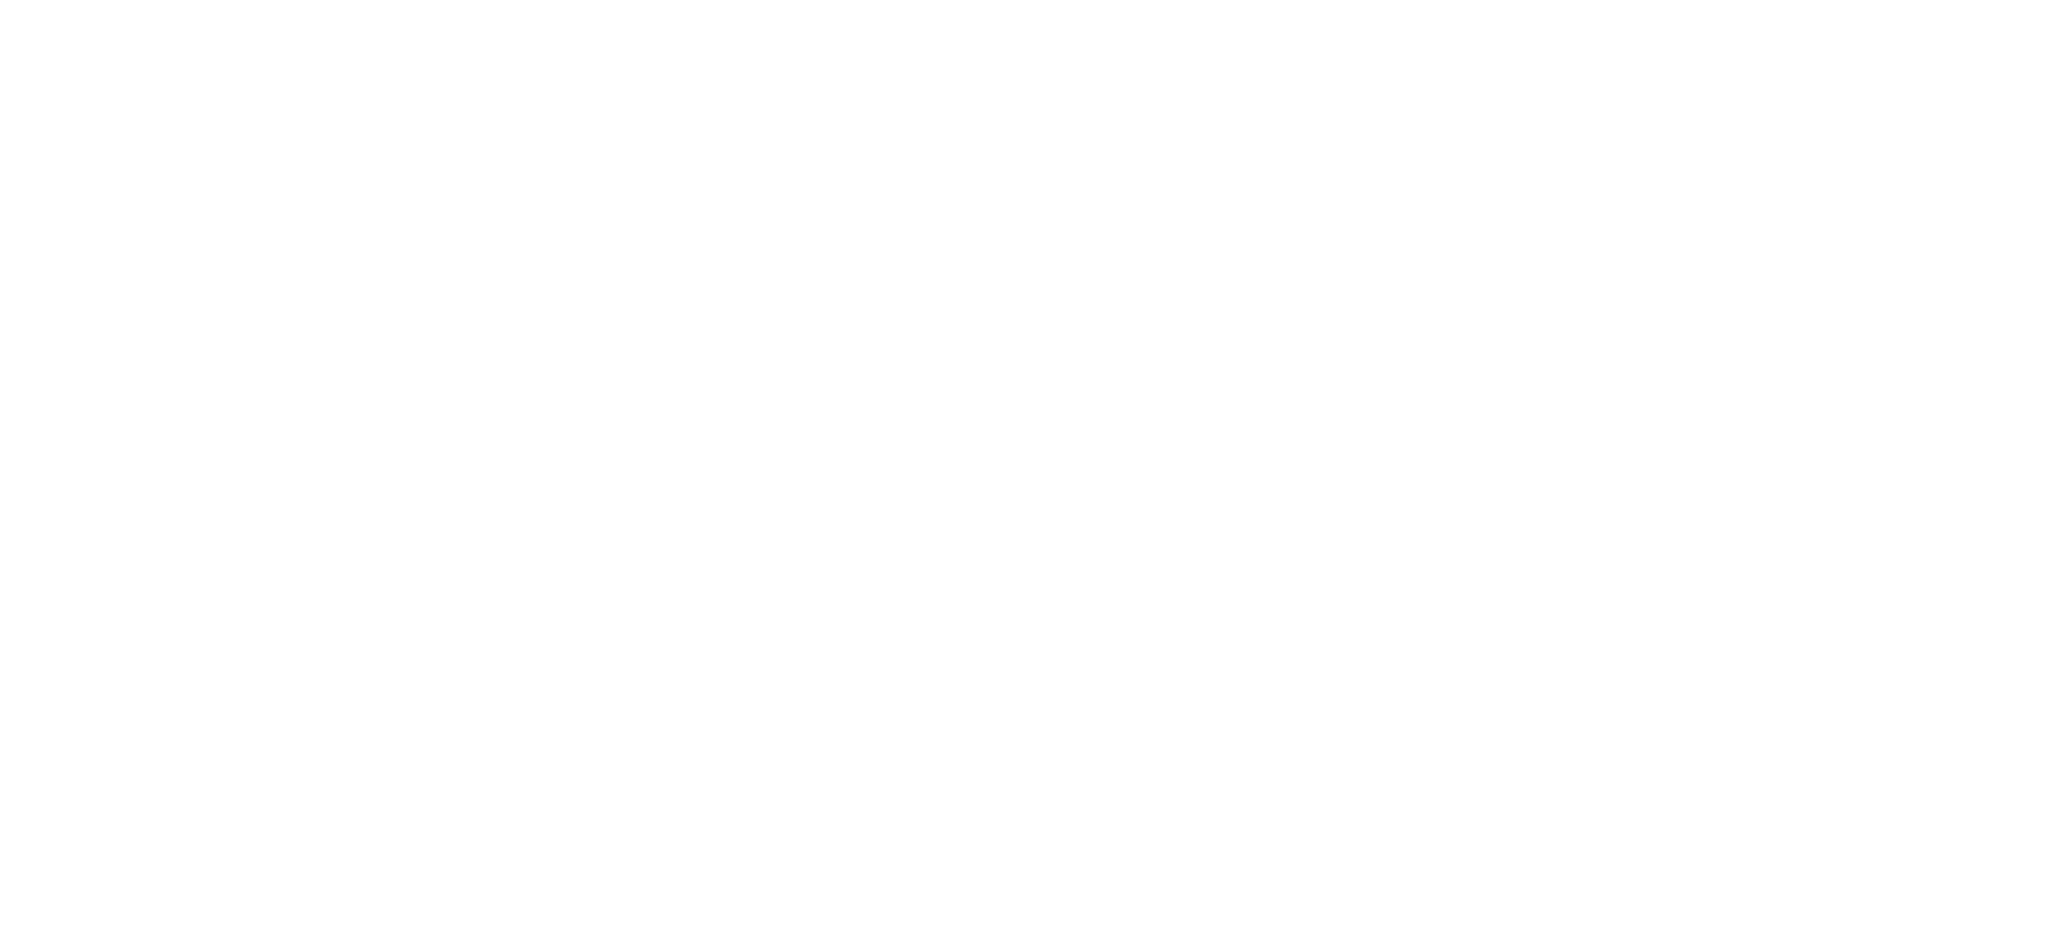
\includegraphics[width=0.85\linewidth]{predictionView}
 \caption{
 In the prediction view, the prediciton probability (the probability of being neutral, contradict, and entailment) is encoded as barycentric coordinate system in an triangle.
 The prediction result for the original sentence pair is represented by larger yellow dot) and their perturbations are illustrated by smaller grey dots.
 A density contour of the prediction is computed to emphasis the highly cluttered areas and distinguish the outliers.
 %How domain experts conduct error analysis on the model.
 }
\label{fig:modelPipeline}
\end{figure}
